\documentclass{report}
\usepackage[T1]{fontenc} % Fontes T1
\usepackage[utf8]{inputenc} % Input UTF8
\usepackage[backend=biber, style=ieee]{biblatex} % para usar bibliografia
\usepackage{csquotes}
\usepackage[portuguese]{babel} %Usar língua portuguesa
\usepackage{blindtext} % Gerar texto automaticamente
\usepackage[printonlyused]{acronym}
\usepackage{hyperref} % para autoref
\usepackage{graphicx}

\usepackage{listings}
\usepackage{color}

\definecolor{dkgreen}{rgb}{0,0.6,0}
\definecolor{gray}{rgb}{0.5,0.5,0.5}
\definecolor{mauve}{rgb}{0.58,0,0.82}

\lstset{frame=tb,
  language=Python,
  aboveskip=3mm,
  belowskip=3mm,
  showstringspaces=false,
  columns=flexible,
  basicstyle={\small\ttfamily},
  numbers=none,
  numberstyle=\tiny\color{gray},
  keywordstyle=\color{blue},
  commentstyle=\color{dkgreen},
  stringstyle=\color{mauve},
  breaklines=true,
  breakatwhitespace=true,
  tabsize=3
}

\bibliography{bibliografia}


\begin{document}
%%
% Definições
%
\def\titulo{Adivinha o Número Secreto}
\def\data{DATA}
\def\autores{Gonçalo Silva, Samuel Teixeira}
\def\autorescontactos{(103) goncalol@ua.pt, (103325) steixeira@ua.pt}
\def\versao{VERSAO 1.0}
\def\departamento{Departamento de Eletrónica, Telecomunicações e Informática}
\def\empresa{Universidade de Aveiro}
\def\logotipo{ua.pdf}
%
%%%%%% CAPA %%%%%%
%
\renewcommand{\contentsname}{Índice}
\begin{titlepage}

\begin{center}
%
\vspace*{50mm}
%
{\Huge \titulo}\\ 
%
\vspace{10mm}
%
{\Large \empresa}\\
%
\vspace{10mm}
%
{\LARGE \autores}\\ 
%
\vspace{30mm}
%
\begin{figure}[h]
\center
\includegraphics{\logotipo}
\end{figure}
%
\vspace{30mm}
\end{center}
%
\begin{flushright}
\versao
\end{flushright}
\end{titlepage}

%%  Página de Título %%
\title{%
{\Huge\textbf{\titulo}}\\
{\Large \departamento\\ \empresa}
}
%
\author{%
    \autores \\
    \autorescontactos
}
%
\date{\data}
%
\maketitle

\pagenumbering{roman}

%%%%%% RESUMO %%%%%%
\begin{abstract}
Este projeto foi realizado no âmbito da cadeira LABI (acr) do 1º ano do MIECT.
Consiste em criar um servidor em que os clientes se conectam para jogar um jogo de
adivinha o número secreto. Para além disso, também tivemos que fazer este mesmo 
relatório em que nós explicamos o projeto: objetivo, motivação, a metodologia utilizada, resultados e
conclusões. Na metodologia, será relatado em pormenor o nosso código feito para criar o servidor, tanto
código do cliente como do servidor, o modo de funcionamento, testagem e comandos git feitos para tal.
Nos resultados, será mostrado o fruto de todo o nosso código que é o servidor a funcionar.
Por fim, nas conclusões, retira-se o que se alcançou com este projeto, o que aprendemos,
o quão útil este projeto é para compreendermos esta matéria da cadeira de LABI e o 
quão interessante foi realizá-lo.
\end{abstract}

%%%%%% Agradecimentos %%%%%%
% Segundo glisc deveria aparecer após conclusão...
\renewcommand{\abstractname}{Agradecimentos}
\begin{abstract}
Queremos agradecer a todos os professores da cadeira de LABI por nos terem dado um trabalho interessante, que nos ajudou a
compreender os conceitos lecionados nas aulas. Queremos também agradecer a Guido van Rossum por ter criado a linguagem Python
e ao Bill Gates por ter sido um dos grandes pilares para a criação de portáteis.

\end{abstract}


\tableofcontents
% \listoftables     % descomentar se necessário
% \listoffigures    % descomentar se necessário


%%%%%%%%%%%%%%%%%%%%%%%%%%%%%%%
\clearpage
\pagenumbering{arabic}

%%%%%%%%%%%%%%%%%%%%%%%%%%%%%%%%
\chapter{Introdução}
\label{chap.introducao}

O objetivo do jogo é que o cliente adivinhe um número secreto entre 0 e 100 criado 
aleatoriamente pelo servidor, dentro de um determinado número de tentativas dadas também
pelo servidor. O cliente tem a possibilidade de realizar quatro operações diferentes. A primeira
serve para iniciar o jogo (START), a segunda serve para tentar adivinhar o número secreto (GUESS), 
a terceira serve para desistir do jogo (STOP) e a última serve para sair (QUIT). O servidor deve responder
adequadamente aquando da operação pretendida. Se houver algum erro, como um cliente inexistente, o 
servidor deve dar uma resposta adequada ao cliente. No final do jogo, o servidor guarda num ficheiro
.csv os dados do cliente que jogou o jogo. Para efeitos de segurança, o cliente possui ainda a
possibilidade de escolher se quer que os seus dados sejam encriptados ou não.

Este documento está dividido em quatro capítulos.
Depois desta introdução,
no \autoref{chap.metodologia} é apresentada a metodologia seguida,
no \autoref{chap.resultados} são apresentados os resultados obtidos,
sendo estes discutidos no \autoref{chap.analise}.
Finalmente, no \autoref{chap.conclusao} são apresentadas
as conclusões do trabalho.


\chapter{Metodologia}
\label{chap.metodologia}
\section{Cliente}
Nesta secção será apresentada a metodologica no ficheiro client.py

\subsection{Função main}
\label{ssec:main}
Devido ao facto do cliente ser invocado com o comando, esses python3 client.py client\_id porto [máquina]"
argumentos têm de ser validados. Para começar, devem ser colocados 3 ou 4 argumentos (máquina é opcional).
Caso não tenha nenhuma destas quantidades, é enviada uma mensagem de erro. Caso o tamanho seja 3, a máquina é
a local(127.0.0.1), caso seja 4 a máquina é o último argumento. 

O client\_id não possui qualquer tipo de restrição, 
logo a única verificação feita é se ele existe (len(argv[1])). Para a porta, existem 2 condições: a porta inserida é 
constituída apenas por números e esse número encontra-se entre 0 e 65535. Para isso, percorre-se todos os caractéres 
da string e, caso não seja um dígito, é enviada uma mensagem de erro.

Por fim, a máquina tem de ser verificada,
os seus números entre cada "." estão compreendidos no intervalo ]0, 255]. Os números são colocados num array através
do método ".split('.')" e, caso algum não satisfaça a condição, é enviada mensagem de erro.

Após esta verificação, é criado o socket com a porta e máquina indicados na invocação, tenta-se estabelecer conexão e chama-se a 
função run\_client, que é onde se vai passar o jogo. Quando terminar, é fechado o socket e o cliente termina.


\subsection{Função run\_client}

\label{ssec:runclient}
A função run\_client é invocada na main. O cliente é introduzido ao jogo e é-lhe questionado se pretende encriptação
de dados (S/N). Enquanto a respotas for diferente dessas duas letras, é enviada uma mensagem de erro. Após a inserção da
opção, é criado um dicionário start com o id e a cifra do cliente. Se foi inserido "S", é criada uma chave que é inserida
no dicionário start na chave cipher. É usada a função sendrecv\_dict do common\_comm como recomendado para enviar start
e receber a resposta do servidor(recvstart). É verificado se houve algum erro no início do jogo através de validate\_response,
se houve termina, senão a variável maxAttempts fica com o valor correspondente em recvstart(desencriptada caso necessário). É escrito no ecrã do cliente as tentativas máximas que tem para adivinhar o número e um menu com as opções que pode fazer
, onde o cliente pode escolher o que fazer. É verificado se o que o cliente inseriu é um número ou não através de um try/except
, onde caso não seja inserido um número, a opção fica com o valor 999 por defeito pois no final da run\_client, essa operação é
 reconhecida como desconhecida e é relatado. Se a opção inserida for 1, é iniciada a operação start, como indicada no menu. 
 
 \begin{figure}[!h]
\center
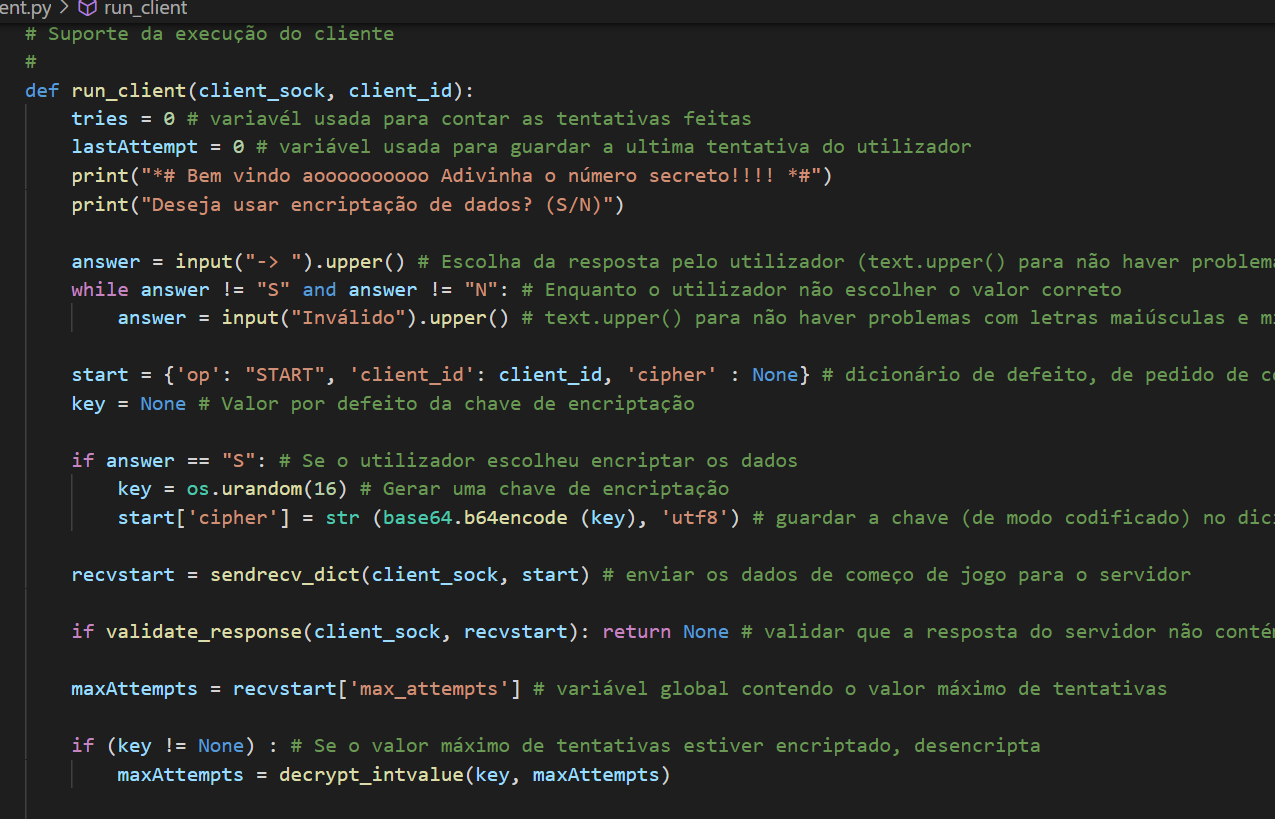
\includegraphics[height = 180pt]{img/run1.png}
\end{figure}

\subsubsection{Opção 1}
\label{sssec:first}

O cliente insere a sua tentativa de adivinhar o número secreto, que é verificada num try/except e, caso seja inválido, dá
erro e é pedida novamente porque encontra-se dentro de um ciclo "while True". Depois de escolhida a opção, é encriptada
caso haja encriptação. É criado um dicionário típico da operação start ({'op': "GUESS", 'number': num}, sendo num a tentativa)
e é enviado para o servidor, recebendo ao mesmo tempo a resposta através de sendrecv\_dict e guardada em recvguess. A resposta é
é validada (validate\_response) e a tentativa é registada em tries. Se o jogador acertou no número, é dito ao cliente e é redirecionado
para a opção 2, se foi maior ou menor ("smaller"/"larger") é também escrito no ecrã esse resultado. Se o número de tentativas
exceder o máximo estipulado pelo servidor, é dito ao cliente e este é redirecionado para a opção 2.

\begin{figure}[!h]
\center
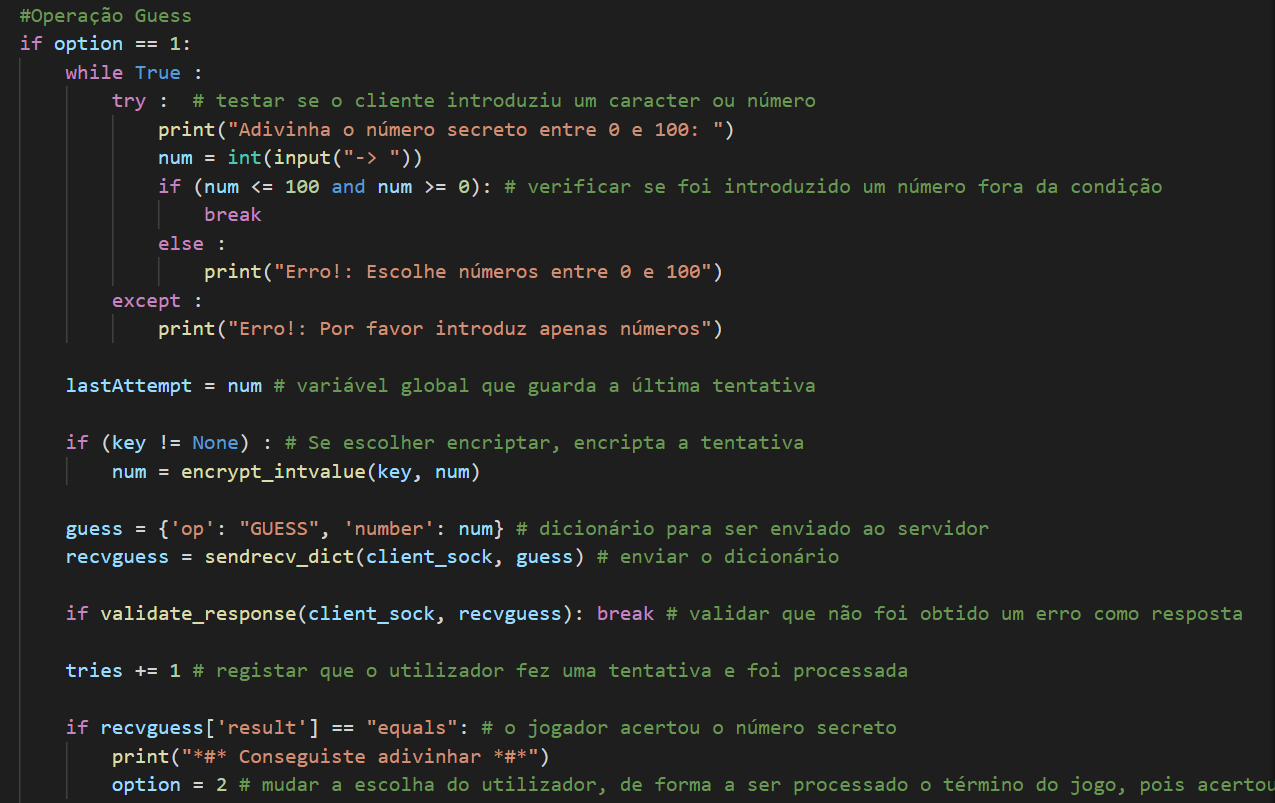
\includegraphics[height = 180pt]{img/option1.png}
\end{figure}
\begin{figure}[!h]
\center
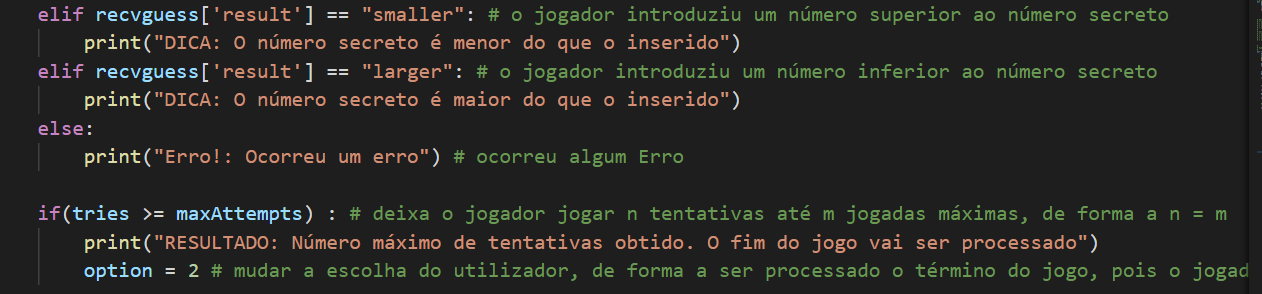
\includegraphics[height = 67pt]{img/opt1sec.png}
\end{figure}
\subsubsection{Opção 2}
\label{sssec:second}

Na opção 2, é guardada a última tentativa do jogador em lastAttempt\_toSend, que é encriptada caso tenha sido escolhida encriptação.
É então criado o diconário típico desta operação ({"op": "STOP", "number": lastAttempt\_toSend, "attempts": tries\_toSend}, sendo
tries\_toSend o número de tentativas feitas). É enviado este dicionário e recebido outro pelo mesmo processo que foi descrito para
a operação 1, só que a resposta é armazenada em recvstop. Essa resposta é validada (validate\_response, caso haja quer dizer que
o jogador excedeu o número de jogadas e perdeu o jogo, é dito ao cliente isso e sai do jogo)
e o número secreto, que está na chave 'guess' de recvstop é armazenada em returnGuess, que é desencriptado se houver encriptação.
Se a última tentativa do jogador for igual ao número secreto, o jogador acertou e ganhou o jogo, senão perdeu. Em ambos os casos
o cliente é informado do seu resultado e sai do jogo.

\subsubsection{Opção 3}
\label{sssec:third}
Na opção 3, o jogador é enviado para a função quit\_action, onde é sistematizada toda a operação esta operação. O output da função
é armazenado em condition. Se condition tiver o valor None, não houve erro e o cliente sai do jogo. Caso contrário, o erro é
dito ao cliente e este sai do jogo.

No fim de todo este código, encontra-se a condição que é executada se o número da operação inserida pelo cliente for inválido. Nessa situação, o cliente é informado deste problema e, visto que tudo isto se encontra dentro de um ciclo "while True", o jogador volta ao menu para escolher outra opção.

\begin{figure}[!h]
\center
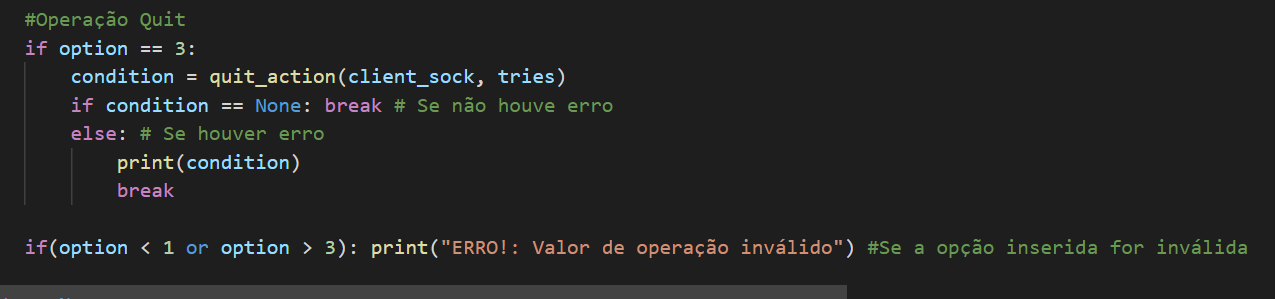
\includegraphics[height = 75pt]{img/option3.png}
\end{figure}
\subsection{Função validate\_response}
\label{ssec:validate}
A função validate\_response procura por uma chave "error" no dicionário response, que corresponde à resposta de um servidor
ao que foi enviado pelo cliente. Visto que, quando existe um erro, seja qual for a operação, esta chave é enviada, é feita essa
procura e, se existir, é enviado um valor booleano True, caso contrário é enviado False

\begin{figure}[!h]
\center
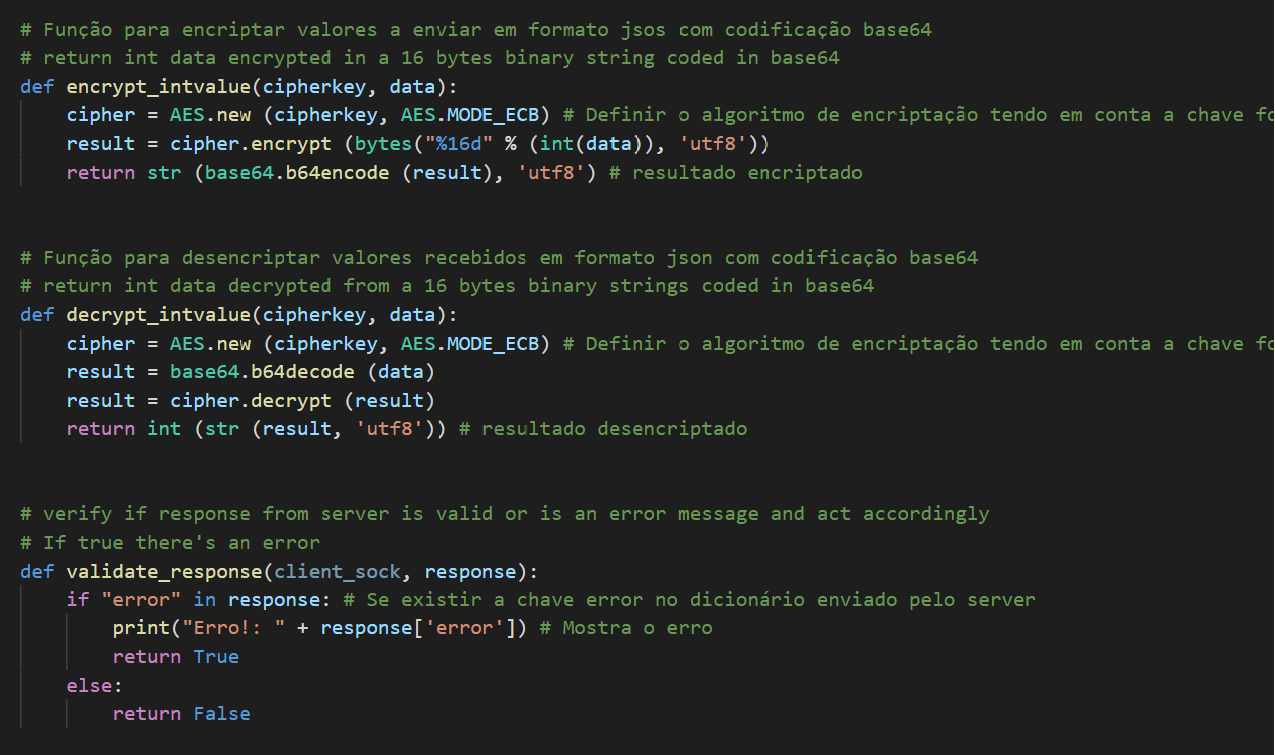
\includegraphics[height = 180pt]{img/cryptovalidate.png}
\end{figure}

\subsection{Função quit\_operation}
\label{ssec:quit}
Nesta função, é criado um dicionário quit com uma única chave com o nome da operação "QUIT". O dicionário recvquit é criado
para receber a resposta do servidor ao enviar quit através de sendrecv\_dict. Se a função validate\_response verificar que existe
um erro, é enviado o return da chave do erro. Se não houver erro, o cliente é informado que desistiu depois de x tentativas,
sendo x "attempts"


\begin{figure}[!h]
\center
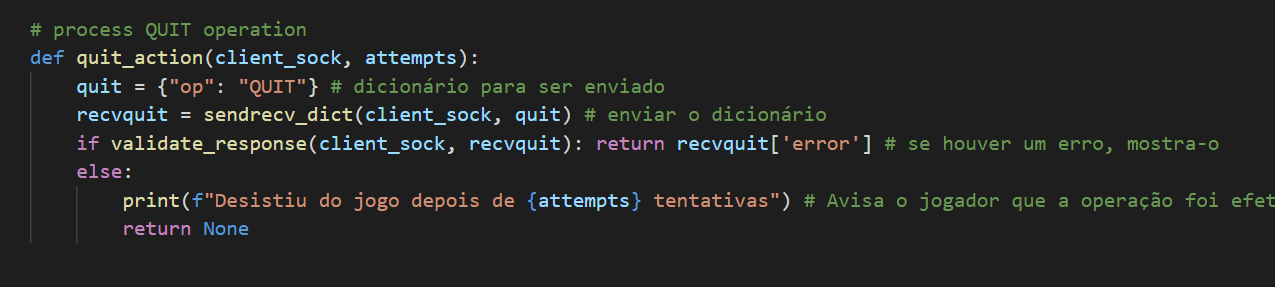
\includegraphics[height = 77pt]{img/quit.png}
\end{figure}
\section{Servidor}
\label{sec:server}
Nesta secção será apresentada e explicada a metodologia docódigo no ficheiro client.py

\subsection{Função main}
\label{ssec:func_main}

A função main é a função principal do cliente e é a primeira a ser executada quando o servidor é iniciado. Para iniciar o servidor, é usado o comando UNIX (ACRÓNIMO) \textbf{'python3 server.py <número do porto>'}. Após o começo do programa, os argumentos de entrada serão validados, começando por verificar se existe um valor do porto e se este é inteiro e está entre 0 e 65535. De seguida o programa tenta iniciar o servidor com a porta fornecida. Se a porta fornecida pelo utilizador for reservada o programa avisa o utilizador e termina, similarmente, se a porta fornecida pelo utilizador já estiver a ser usada por um outro servidor a correr, o programa irá comunicar ao utilizador e terminar. 

Caso não exista nenhum erro nas condições acima, o servidor irá ser iniciado e criará o ficheiro de resultados dos jogadores "report.csv", bem como passará a ficar "à escuta" de conecções dos clientes.

Com o servidor a funcionar, este vai ficar à espera de conecções de clientes. Quando um cliente tentar se conectar, o servidor irá obter os valores do seu socket e verificar se já existe algum cliente na lista com os mesmos valores, se não existir, então irá adicioná-lo à lista.

Tendo o cliente estabelecido a conecção com sucesso, este irá comunicar com o servidor através de pedidos. Esses pedidos são "ouvidos" pelo servidor e comunicados à \nameref{ssec:func_new_msg} que os irá processar.

Finalmente, como estão a ser usados sockets TCP (ACRÓNIMO), estes "sentem" se alguma exceção aconteceu e se o cliente se desconectou do servidor, caso isso aconteça, o servidor irá remover este cliente da lista de clientes, executar a \nameref{ssec:func_clean_client} e fechar o socket do cliente.

\subsection{Função find\_client\_id}
\label{ssec:func_find_client_id}

A função find\_client\_id aceita como parâmetros o socket do cliente e procura se este se encontra registado no dicionário de jogadores ativos, gamers e devolve o id do cliente que está associado. Caso contrário devolve "None", indicando que não existe nenhum cliente associado.

\subsection{Função encrypt\_intvalue}
\label{ssec:func_encrypt_value_server}

O objetivo desta função é encriptar um valor inteiro, para tal, aceita como parâmetros o id do cliente e um valor inteiro, devolvendo uma palavra (String) codificada que representa esse valor. De seguida, é usada a chave previamente guardada no dicionário associada ao id do cliente e criada uma cifra do tipo AES-128 (ACRONIMO). Esta crifa criada, será usada para encriptar o número em forma de bytes do tipo 'utf8'. Por final, convertemos os bytes que obtivemos no passo anterior para texto (String) usando a função \textbf{base64.b64encode} (Acrónimo).

\subsection{Função decrypt\_intvalue}
\label{ssec:func_decrypt_value_server}

O funcionamento desta função é próximo ao da \nameref{ssec:func_encrypt_value_server}, tendo apenas o funcionamento oposto. Para desencriptar os números, a função aceita como parâmetros o id do cliente e um texto (String). Começa por criar a chave de encriptação do tipo AES-128 (ACRONIMO) e de seguida converte o texto que recebemos em bytes usando a função \textbf{base64.b64decode} (Acrónimo). Tendo obtido o valor em bytes, procede à desencriptação usando a cifra criada anteriormente. Por fim, converte os valores bytes obtidos em uma String desencriptada, convertendo essa String para inteiro e devolvendo-a.

\begin{figure}[!h]
\center
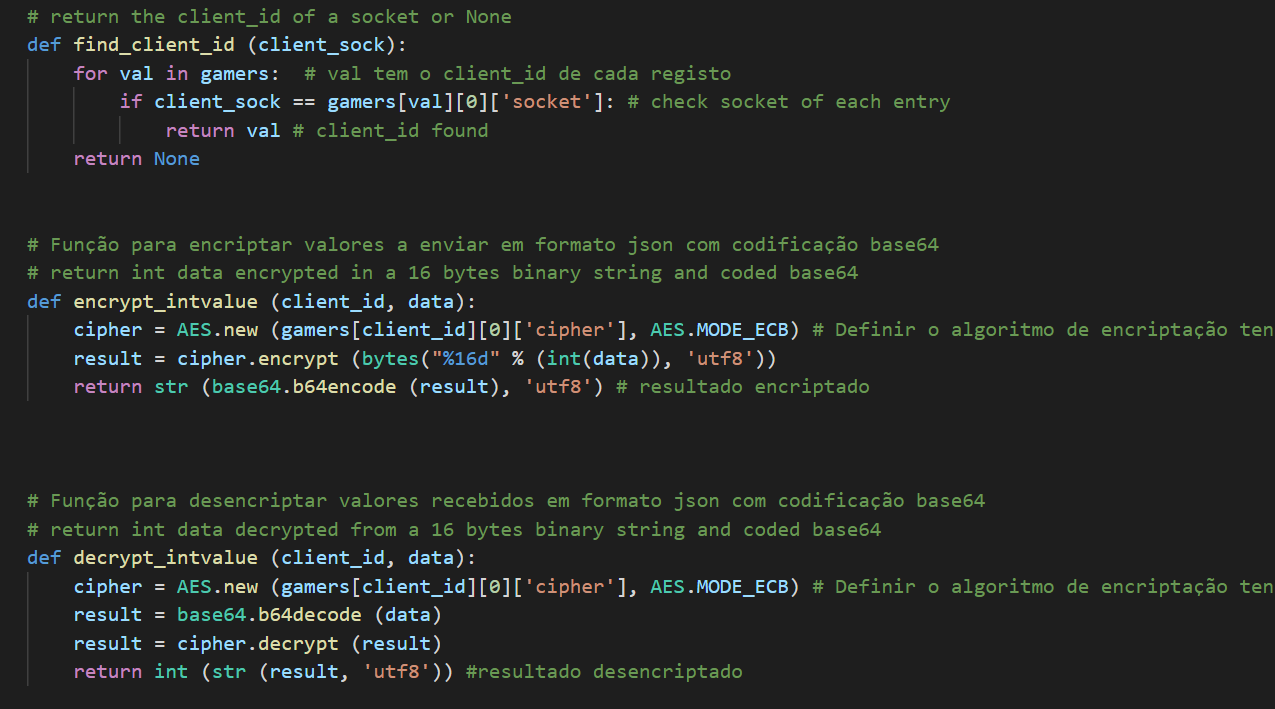
\includegraphics[height = 180pt]{img/cryptofindid.png}
\end{figure}

\subsection{Função new\_msg}
\label{ssec:func_new_msg}

A função new\_msg é usada como um centro de processamento das mensagens enviadas pelo cliente. QUando um cliente envia um pedido de processamento para o servidor, precisa de conter o campo 'op' que corresponde à operação escolhida pelo utilizador, caso este campo não exista no pedido do cliente, ou apresenta uma operação inválida, o servidor envia uma resposta de erro ao cliente.

Se o cliente enviou um pedido corretamente formulado ao servidor, este pode processar quatro tipos de mensagens:
\begin{itemize}
\item \textbf{'START'} - Pedido do começo do jogo (\nameref{ssec:func_new_client})
\item \textbf{'QUIT'} - Processar a desistência do jogador (\nameref{ssec:func_quit_client})
\item \textbf{'GUESS'} - Processar a adivinha do jogador (\nameref{ssec:func_guess_client})
\item \textbf{'STOP'} - Processar o término do jogo (\nameref{ssec:func_stop_client})
\end{itemize}
Cada uma destas operações devolve uma resposta para ser enviada ao cliente, dependendo da operação e do seu sucesso. Por fim, tendo processado a resposta ao pedido do cliente, a função o seu resultado ao cliente. 

\begin{figure}[!h]
\center
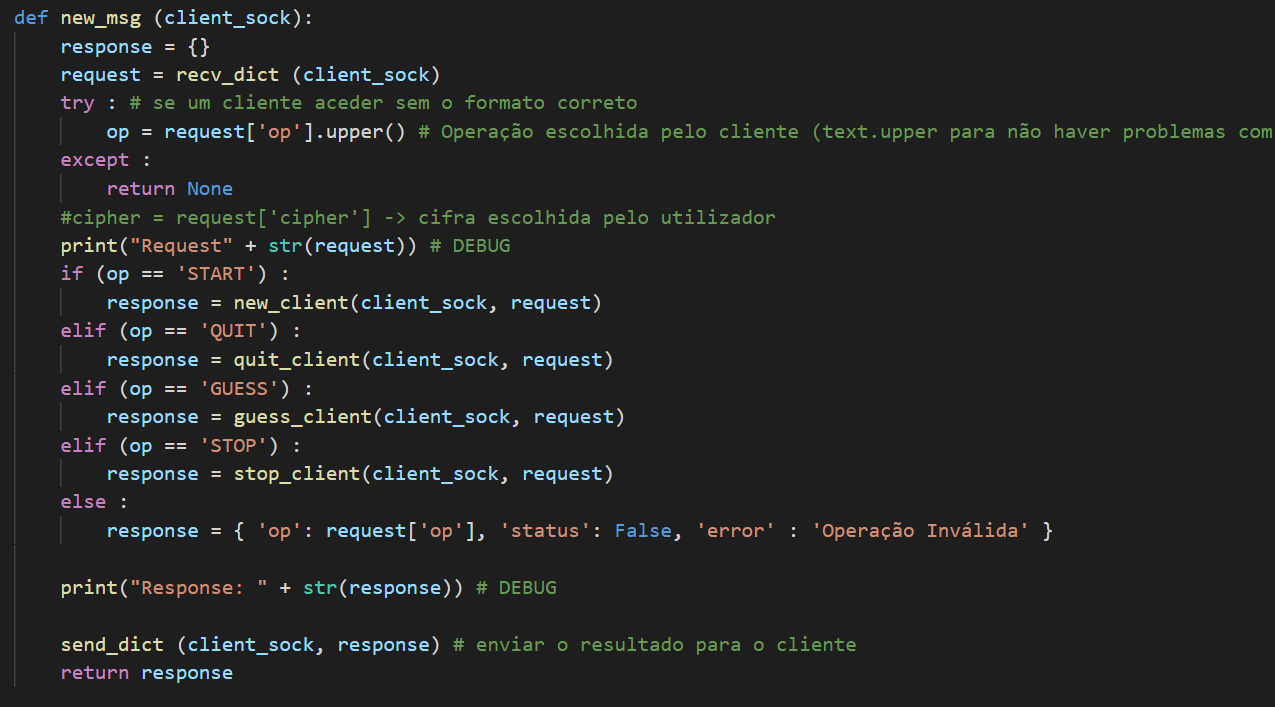
\includegraphics[height = 180pt]{img/newmsg.png}
\end{figure}

\subsection{Função new\_client}
\label{ssec:func_new_client}

A função new\_client processa o pedido de começo de jogo do cliente, devolvendo um dicionário com o número máximo de tentativas, cajo seja processada com sucesso. Se a função não for processada com sucesso, significa que o cliente não está inscrito como como jogador ativo. A função aceita como parâmetros de entrada o socket do cliente e o pedido do jogador.

Além das verificação faladas acima, a função também verifica se o jogador enviou os campos necessários para efetuar o pedido, nomeadamente o campo "client\_id".

Se o formato do pedido estiver correto e o cliente existir, a função irá gerar o número secreto para o jogador adivinhar e o número máximo de jogadas. De seguida adicionará o cliente à lista de jogadores ativos e terá em conta se foi escolhido encriptação, tomando as ações necessárias para encriptar os dados. recorrendo à função  \nameref{ssec:func_encrypt_value_server}.

\begin{figure}[!h]
\center
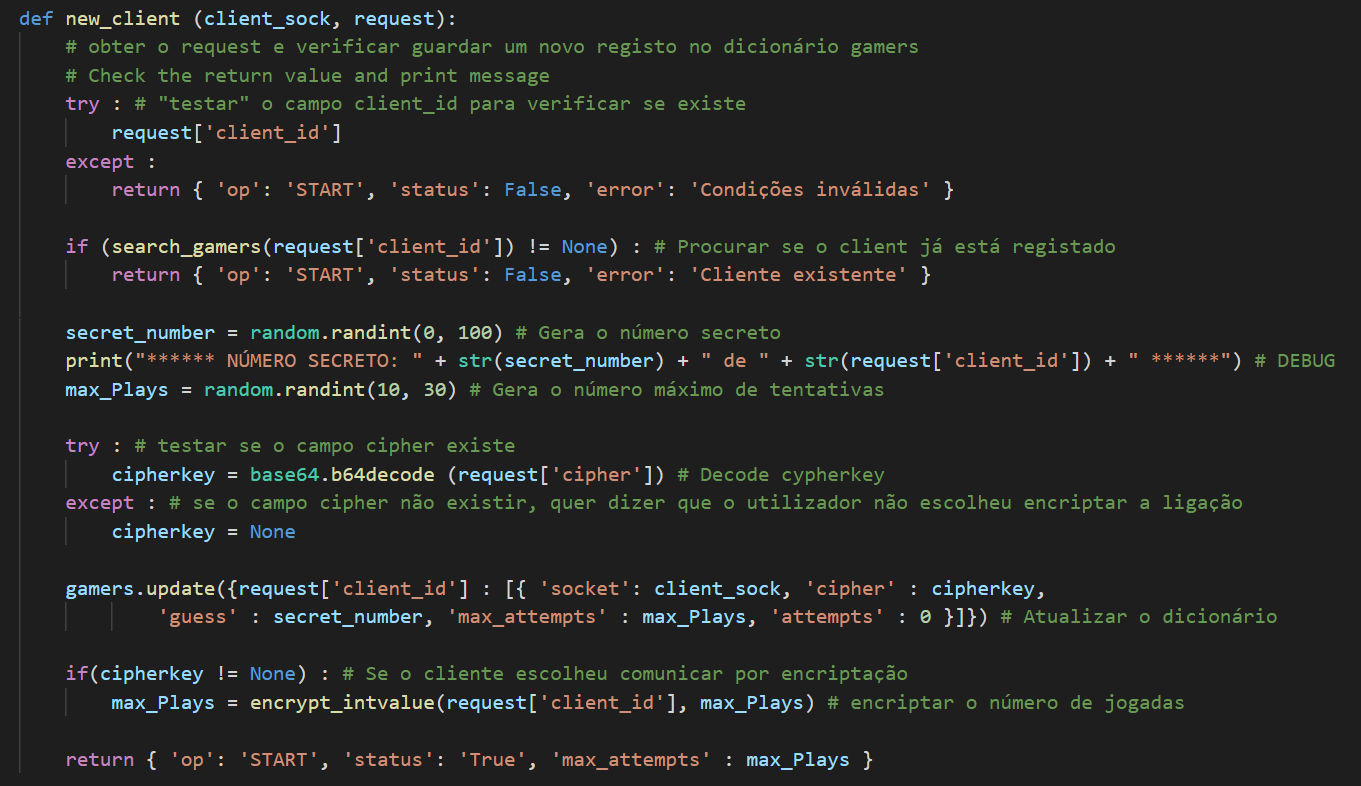
\includegraphics[height = 180pt]{img/newclient.png}
\end{figure}

\subsection{Função clean\_client}
\label{ssec:func_clean_client}

Esta função tem como objetivo, eliminar o cliente da lista de jogadores ativos, para isso, aceita como parâmetro o socket do cliente e procura o id do mesmo. Se o o id não existir, significa que o cliente não está registado, retornando "False". Caso esteje registado, então apaga-o do dicionário de jogadores ativos e devolve "True".

\begin{figure}[!h]
\center
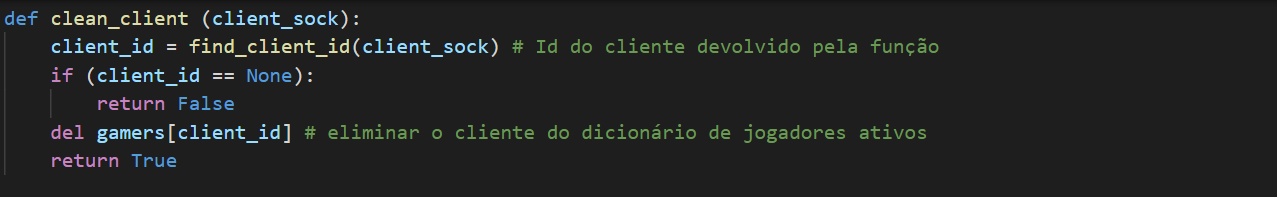
\includegraphics[height = 53pt]{img/cleanclient.png}
\end{figure}

\subsection{Função quit\_client}
\label{ssec:func_quit_client}

A função quit\_client processa a operação de desistência do jogo, tendo como pré-requisito a existência de o cliente na lista de jogadores ativos e o formato de pedido de operação correto.

Tendo estas condições sido verificadas, o servidor irá processar a desisência do cliente, recorrendo à \nameref{ssec:func_update_file} para atualizar os dados do cliente e à \nameref{ssec:func_clean_client} para remover o cliente da lista de jogadores ativos.

Se o pedido tiver sido processado corretamente, a função retornará o sucesso da mesma, caso contrário devolverá o erro sucedido.

\subsection{Função create\_file}
\label{ssec:func_create_file}

Esta função é usada para criar o ficheiro "Report.csv" que posteriormente será usado para guardar os resultados dos jogos dos cliente, quando estes o terminam.

\subsection{Função update\_file}
\label{ssec:func_update_file}

A função update\_file é usada para atualizar o ficheiro "Report.csv" com os resultados dos jogos dos clientes. Tem como parâmetros o id do cliente e o a linha de dados para serem acrescentados.

A função abre o ficheiro em modo de append, para não sobrescrever os dados, mas sim para acrescentar mais uma linha com resultados ao ficheiro.

\begin{figure}[!h]
\center
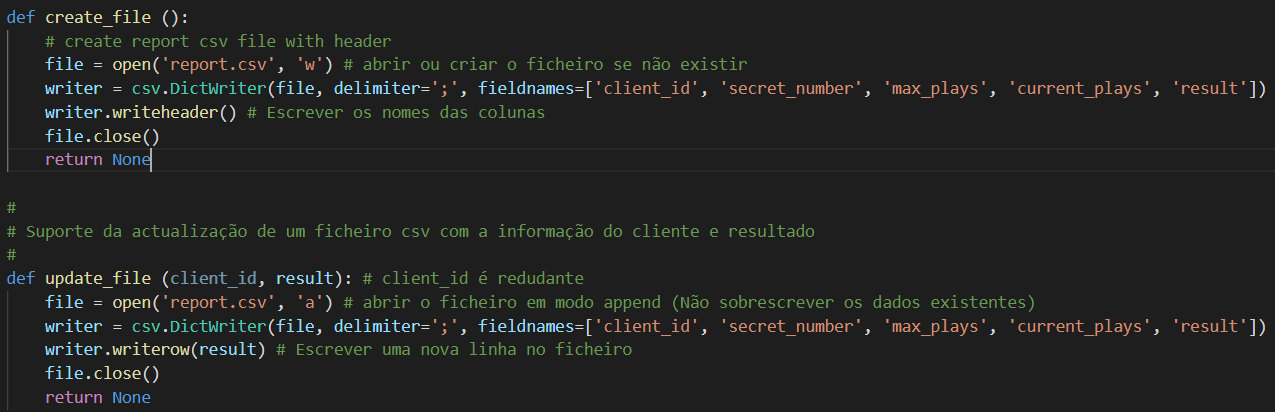
\includegraphics[height = 110pt]{img/createupdate.png}
\end{figure}

\subsection{Função guess\_client}
\label{ssec:func_guess_client}

Para o cliente efetuar uma tentativa do número secreto, é usada a função guess\_client, que aceita como parâmetros de entrada o socket do cliente e o pedido.

Antes de efetuar a operação de guess, a função verifica se existe um jogador ativo com o socket fornecido e se o campo "number" foi fornecido no pedido do cliente.

Se as condições anteriores forem verificadas, o servidor contará uma tentativa realizada e caso o cliente tenha escolhido encriptação de dados, irá desencriptar o campo "number", recorrendo à \nameref{ssec:func_decrypt_value_server}. Após ter o valor da tentativa, o servidor irá comparar o número da tentativa com o número secreto que tem armazenado e irá devolver um dos três resultados:
\begin{itemize}
\item \textbf{'larger'} - Se o cliente escolheu um número inferior ao número secreto;
\item \textbf{'smaller'} - Se o cliente escolheu escolheu um número superior ao número secreto;
\item \textbf{'equals'} - Se o cliente acertou o número secreto;
\end{itemize}

\subsection{Função stop\_client}
\label{ssec:func_stop_client}

A função stop\_client processa o término do jogo. Aceita como parâmetros de entrada, o socket do cliente e o pedido do cliente.

Para processar a operação, a função garante que existe um jogador ativo, com o socket fornecido, usando a  \nameref{ssec:func_find_client_id} e se os campo "attempts" e "number" foram fornecido no pedido do cliente. Além disso, a função também levará em conta se estes campos fornecidos estão encriptados, se estivrem, irá utilizar a \nameref{ssec:func_decrypt_value_server} para proceder à desencriptação.

Caso as condições anteriores se verifiquem, o servidor vai dar inicio ao processamento do término do jogo. Se o cliente \textbf{não} tiver enviado um número correto de tentativas ou exceder o número máximo de tentativas, o servidor vai enviar a mensagem de \textbf{erro} "Número de jogadas inconsistente". Caso contrário, verifica se o cliente acertou o jogo. Se o cliente tiver acertado o número secreto, envia dicionário com o número secreto para o utilizador e guarda que o cliente acertou, caso contrário, envia também o dicionário para o cliente, mas guarda que o cliente falhou o número secreto.

Após as verificações anteriores, o servidor irá atualizar o ficheiro 'report.csv' usando a \nameref{ssec:func_update_file} escolhendo o campo "Result" como "SUCCESS" ou "FAILURE", se o jogador acertou ou falhou o número secreto ou apresenta um número de jogadas inconsistente, respetivamente.

Por fim, o servidor desvincula o client, recorrendo à \nameref{ssec:func_clean_client} e remove o cliente da lista de jogadores ativos.

\begin{figure}[!h]
\center
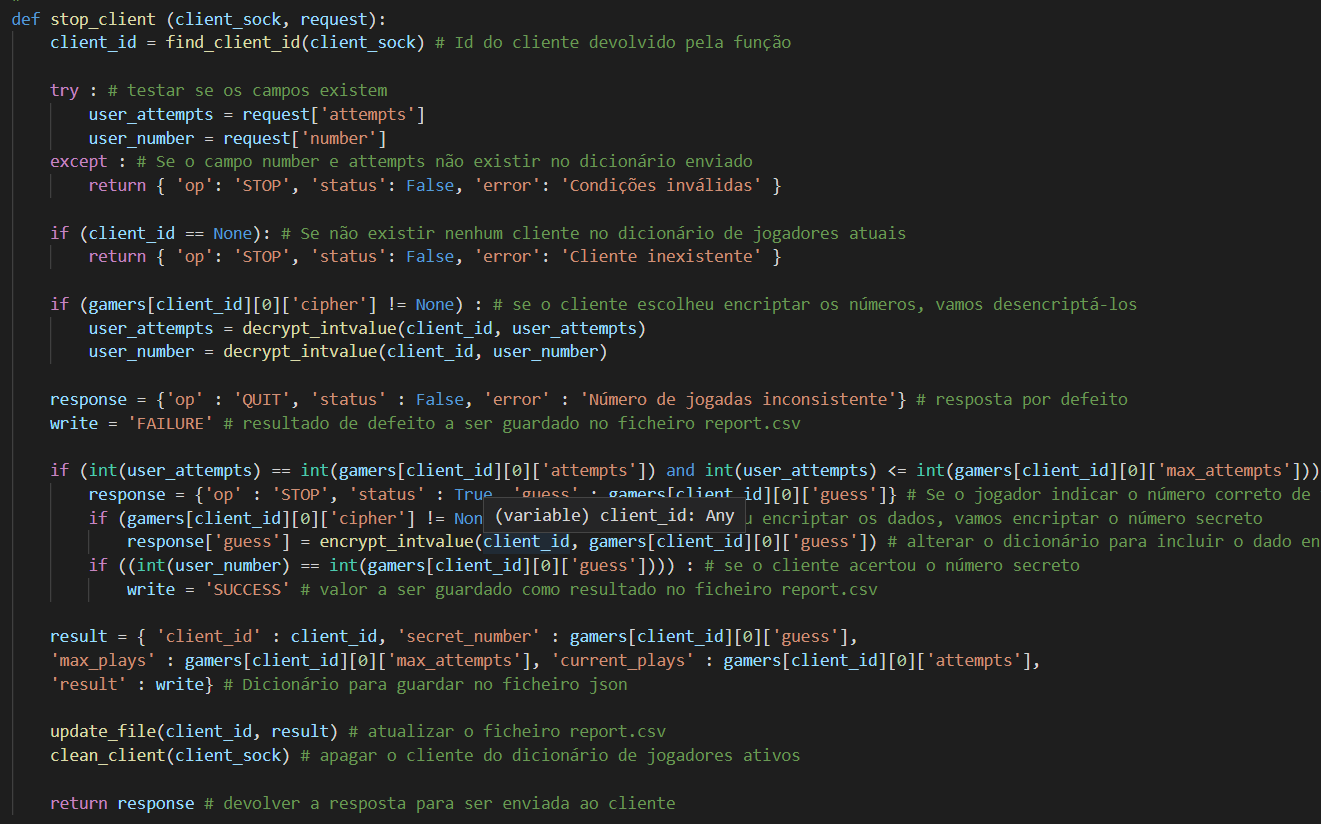
\includegraphics[height = 200pt]{img/stopclient.png}
\end{figure}

\section{Git}
\label{sec:git}
As funcionalidades do git foram muito utilizados neste projeto, desde a simples sincronização de ficheiros e código, até à criação, junção e gestão de branches (\textbf{IMAGEM DE EXEMPLO})

\section{Code UA}
\label{sec:git}
As funcionalidades do Code UA forneceram bastante ajuda ao desenvolvimento projeto, desde a própria visualização dos branches disponíveis, bem como a própria gestão e visualização do código, até à criação de funcionalidades a serem desenvolvidas e bugs a serem resolvidos. Pode visualizar o projeto no Code UA, através do link: http://code.ua.pt/projects/labi2021-ap2-g29


\section{Exemplos}


\chapter{Resultados}
\label{chap.resultados}
Descreve os resultados obtidos.

\chapter{Análise}
\label{chap.analise}
Analisa os resultados.

\chapter{Conclusões}
\label{chap.conclusao}
Com este trabalho, conseguimos solidificar o nosso conhecimento de servidores em python, sockets, interações entre 
cliente e servidor e criação de algoritmos para tal, bem como encriptação e desencriptação de dados para uma partilha
de informação mais segura. Houve também uma aproximação à linguagem Python e a toda à sua sintaxe e características.
Sendo Python uma linguagem com bastante procura no mercado de trabalho, a criação do servidor veio ajudar a compreender
a sua autenticidade e pas suas diferenças em relação a outras linguagens com que já estamos habituados (Ex: Java)
Apesar das adversidades, acreditamos que o trabalho foi conseguido com sucesso, conseguimos criar um servidor 
com o jogo referido e com todas as características necessárias para tal, utilizando os recursos que nos foram dados
e auxiliando a sua compreensão com este relatório.

\chapter*{Contribuições dos autores}
Resumir aqui o que cada autor fez no trabalho.
Usar abreviaturas para identificar os autores,
por exemplo AS para António Silva.
No fim indicar a percentagem de contribuição de cada autor.

%%%%%%%%%%%%%%%%%%%%%%%%%%%%%%%%%
\chapter*{Acrónimos}
\begin{acronym}
\acro{ua}[UA]{Universidade de Aveiro}
\acro{miect}[MIECT]{Mestrado Integrado em Engenharia de Computadores e Telemática}
\acro{lei}[LEI]{Licenciatura em Engenharia Informática}
\acro{glisc}[GLISC]{Grey Literature International Steering Committee}
\end{acronym}


%%%%%%%%%%%%%%%%%%%%%%%%%%%%%%%%%
\printbibliography

\end{document}
